\section{Initial-state matching in the supplied input decks}
\label{sec:initialization}

The source compares a relativistic PIC calculation with nonrelativistic
ten-moment fluid calculations and describes their common initialization in
Appendices A and C~\cite{original}. The deposited reference-case decks and
initial moments make the physical matching of those states directly
testable~\cite{dataset}. Equal numerical drift and temperature parameters
need not specify equal laboratory-frame velocity moments in the two codes.
This issue concerns the controlled comparison; the mixture identities do
not depend on either code's initialization convention.

\subsection{A proper-momentum parameter is used as a fluid velocity}
The PIC deck sets \texttt{use\_spatial\_ufl=.true.} and supplies the curl-derived
drift expressions as \texttt{spatial\_ufl}. The official OSIRIS reference
defines these inputs as proper velocities, or momentum divided by particle
mass, with relativistic boosting as the default~\cite{osirisudist}.
No classical-addition override appears in the posted deck. The Lua decks
instead set nonrelativistic conserved momentum density to $\rho\mathbf v$
using the same expressions. This is the ordinary velocity variable of the
ten-moment equations~\cite{wang2015}.

Writing $\mathbf U=\mathbf p/(m_ec)$, a cold population with proper drift
$\mathbf U$ has
\begin{equation}
 \frac{\mathbf v}{c}=\frac{\mathbf U}{\sqrt{1+|\mathbf U|^2}}.
 \label{eq:proper-ordinary}
\end{equation}
Thus the same numerical vector used for $\mathbf U$ in PIC and $\mathbf v/c$
in the fluid initializer does not match the physical cold drift. At the
unperturbed lower sheet center, the reference expressions give approximately
$(0,0,0.5)$: the cold PIC speed is $0.4472136c$, whereas the prescribed fluid
speed is $0.5c$. The fractional difference is $10.56\%$. It persists when
the thermal spread tends to zero at fixed $B_{\mathrm{Reconn.}}=0.5$ and sheet
width $d_e$; low thermal beta alone does not remove it. Equation
\eqref{eq:proper-ordinary} is a cold-limit explanation. A finite-temperature
mean must be measured after loading rather than identified with that limit.

\subsection{A conditional finite-temperature loading calculation}
The complete 155-line posted PIC deck contains two thermal-distribution
blocks with $\sigma=0.111803$, and no classical-addition override or include
directive. The inspected public OSIRIS loader draws independent Gaussian
thermal proper-momentum components and boosts each particle without changing
its weight~\cite{osirisloader}. With $c=1$, for thermal momentum
$\mathbf w\sim\mathcal N(0,\sigma^2I)$ and proper drift $\mathbf U$, this rule is
\[
 \gamma_0=\sqrt{1+|\mathbf w|^2},\quad G=\sqrt{1+|\mathbf U|^2},\quad
 \mathbf p=\mathbf w+\mathbf U
 \left(\gamma_0+\frac{\mathbf w\cdot\mathbf U}{G+1}\right),\quad
 \mathbf v=\frac{\mathbf p}{G\gamma_0+\mathbf w\cdot\mathbf U}.
\]
This is a prediction conditional on the public loading rule, not an
identification of the original executable. With $\beta=|\mathbf U|/G$ and
$z=w_\parallel/\gamma_0$, pairing opposite Gaussian momenta gives
\[
 \mathbb E[v_\parallel]
 =\beta\left[1-(1-\beta^2)
 \mathbb E\left(\frac{z^2}{1-\beta^2z^2}\right)\right]<\beta
\]
for positive drift and nonzero thermal spread. Thus the mean can fall below
the cold conversion without an additional force. An invariant scalar
distribution sampled at equal laboratory time would require a different
Jacobian-weighted measure; it must not be silently substituted for this
unweighted sample-boost rule.

At $\mathbf U=(0,0,0.5)$ the finite-temperature mean is $0.44297014c$,
below the cold $0.44721360c$. Evaluating the full spatial drift expressions
and perturbations at the two lower diagnostic rows gives an $x$-averaged
zero-shape prediction $0.44197416c$. A separate, unfitted sensitivity uses
the declared quadratic interpolation, the recorded moment-cell offset and
the posted $25\times25$ regular particle lattice. Summing the standard
quadratic weights over their support gives the following conditional values:
\begin{center}
\begin{tabular}{lrr}
\toprule
Quantity & $Y=15.95d_e$ & $Y=16.05d_e$ \\
\midrule
Archived $\overline v_z/c$ & 0.44098722 & 0.44087669 \\
Pointwise loading prediction & 0.44197416 & 0.44197416 \\
Quadratic-shape prediction & 0.44098868 & 0.44098868 \\
Archived $P_{xx}$ & 0.00994868 & 0.00997543 \\
Quadratic-shape $P_{xx}$ & 0.00996490 & 0.00996490 \\
Archived $P_{zz}$ & 0.00769653 & 0.00769303 \\
Quadratic-shape $P_{zz}$ & 0.00770632 & 0.00770632 \\
\bottomrule
\end{tabular}
\end{center}
These pressure predictions use expected raw moments centered at each node
before averaging, in the infinite-particle limit. No temperature, drift,
shape width or perturbation is fitted to the archived values. Quadrature
orders 12, 20, 32 and 48 agree in the quadratic mean to about
$5\times10^{-16}c$; an independent Cartesian quadrature checks the reduced
moment calculation to $1.73\times10^{-15}$ in the tested quantities.
This is a conditional consistency check of the scale of the additional
reduction below the cold value. Agreement does not identify the historical
loader or the custom diagnostic kernel.
The standard public deposition kernel is not verified as the original
custom velocity diagnostic's kernel, so the pointwise prediction and shape
sensitivity remain distinct. Neither is a new PIC run or a confidence
statement about the unidentified original build.

\subsection{Archived initial current and staggered magnetic curl}
The original data authors explicitly define the archived diagnostic
\texttt{vfl\_i} as $(1/n)\int f v_i\,\dd^3v$~\cite{dataset}.
It is therefore an ordinary mean velocity, even though the input parameter
\texttt{ufl} is a proper-momentum parameter. With the source normalization
$q_e=-1$, the physical moment current is
\begin{equation}
 J_z^{\mathrm{mom}}=-\left(n_1\overline v_{1z}+n_2\overline v_{2z}\right).
 \label{eq:archived-moment-current}
\end{equation}
The selected initial density diagnostics give $n_1+n_2=1$ to within
$1.5\times10^{-8}$. No particle tracking or new time integration is needed
to evaluate this current.

The HDF5 files also record their grid offsets: density and velocity moments
have $(0.5,0.5)$, $B_x$ has $(0.5,1)$ and $B_y$ has $(1,0.5)$.
The backward staggered differences therefore place
\begin{equation}
 J_{z,i,j}^{B}=
 \frac{B_{y,i,j}-B_{y,i-1,j}}{\Delta x}
 -\frac{B_{x,i,j}-B_{x,i,j-1}}{\Delta y},\qquad
 \Delta x=\Delta y=0.1d_e,
 \label{eq:archived-magnetic-curl}
\end{equation}
on the moment-cell centers. Periodic differencing makes the first term's
$x$ average exactly zero. The raw data use $y\in[-32,32]d_e$; the paper's
coordinate is $Y=y+32d_e$, so its lower sheet is at $Y=16d_e$.

\begin{table}[htbp]
\centering
\caption{Initial $x$-averaged currents in the cells adjoining the lower sheet.
The deficit is $1-\langle J_z^{\mathrm{mom}}\rangle_x/
\langle J_z^B\rangle_x$. Currents use the source's normalized units.}
\label{tab:initial-current}
\begin{tabular}{rrrr}
\toprule
$Y/d_e$ & $\langle J_z^{\mathrm{mom}}\rangle_x$ &
$\langle J_z^B\rangle_x$ & Deficit \\
\midrule
15.95 & $-0.44098723$ & $-0.49833998$ & $11.5088\%$ \\
16.05 & $-0.44087669$ & $-0.49833998$ & $11.5309\%$ \\
\bottomrule
\end{tabular}
\end{table}

The supplied fluid initializer prescribes an $x$-averaged ordinary velocity
$0.49875256c$ in these same cells. The archived PIC means are
$0.44098722c$ and $0.44087669c$, approximately $11.6\%$ smaller. The small
difference between this continuum prescription and Table~\ref{tab:initial-current}'s
staggered curl does not explain the observed deficit. The adjacent cells at
the other sheet show the same effect with reversed current sign.

The result is not restricted to these four illustrative cells.
Across all 640 rows, the relative $\ell^2$ discrepancy between the
$x$-averaged moment-current and Yee-curl profiles is $9.8265\%$.
Restricting to $14\leq Y/d_e\leq18$ or $46\leq Y/d_e\leq50$ gives
$9.8287\%$ and $9.8408\%$, respectively. These are norms of the
one-dimensional averaged profiles, not norms of the full two-dimensional
fields. Figure~\ref{fig:full-profile} displays both sheets and the full domain.
The input-prescribed current differs from the Yee profile by only $0.0630\%$
in the full-profile relative norm.

As a deterministic discretization sensitivity, averaging the staggered fields
onto cell centers before a centered derivative changes the curl profile by
$0.3755\%$ in that norm. This is a deliberately smoothed representation,
not an alternative reading of the recorded Yee offsets. The central-cell
moment-current deficits remain about $11.05$--$11.10\%$ against that smoothed
profile. Eight contiguous 60-column blocks at $Y=15.95d_e$ have moment-current
means between $-0.4417104$ and $-0.4404351$, compared with the Yee mean
$-0.4983400$. The per-column standard deviation is $0.0019906$.
These spatial summaries are descriptive; correlated particle deposition and
the imposed perturbation preclude treating them as independent-sample
confidence intervals.

Here $J_z^{\mathrm{mom}}$ is a moment-based physical diagnostic. We have not
reloaded OSIRIS's native charge-conserving deposited current, which can differ
from a simple $qv$ deposition. These numbers therefore do not specify the
exact discrete electric-field update of the original executable.
In the normalized continuum equations,
$\partial_t E_z=(\nabla\times\mathbf B)_z-J_z$.
The comparison is a continuum magnetostatic diagnostic. It does not establish
an initial transient in the native numerical electric-field update.

\subsection{The laboratory-frame pressure moments also differ}
The record defines its second-moment diagnostics without a density
normalization: $M_{s,ii}=\int f_s v_i^2\,\dd^3v$~\cite{dataset}.
Following the source's own pressure definition, at $m_e=1$ we compute
\begin{equation}
 P_{ii}=M_{1,ii}+M_{2,ii}-n\overline v_i^2.
 \label{eq:archived-pressure}
\end{equation}
The posted fluid initializers prescribe an isotropic thermal pressure
\[
p_{\mathrm{fl}}=n_0(0.111803)^2=0.012499910809.
\]
The archived initial fluid \texttt{.bp} fields independently confirm this
pressure in both fluid models, as detailed below. The measured ratios to
the archived fluid pressure are
\begin{center}
\begin{tabular}{rrr}
\toprule
$Y/d_e$ & $\langle P_{xx}\rangle_x/p_{\mathrm{fl}}$ &
$\langle P_{zz}\rangle_x/p_{\mathrm{fl}}$ \\
\midrule
15.95 & 0.795900 & 0.615727 \\
16.05 & 0.798040 & 0.615447 \\
\bottomrule
\end{tabular}
\end{center}
For example, at $Y=15.95d_e$ the archived values are
$\langle P_{xx}\rangle_x=0.00994868$ and
$\langle P_{zz}\rangle_x=0.00769653$. The latter is about $38.4\%$ below
the archived fluid pressure. These are the ordinary-velocity covariance
moments defined in the source, not components of a relativistic
energy--momentum tensor. A common rest-frame thermal-momentum parameter
does not imply equal laboratory-frame velocity covariance after a boost.
Centering the pressure after averaging in $x$ instead adds the
density-weighted variance of the resolved mean flow. At the four central
rows this changes either diagonal component by approximately
$4\times10^{-6}$, far smaller than the reported pressure mismatch;
the source definition and our principal result center each cell first.
Figure~\ref{fig:initial-state} shows the local $x$-averaged profiles.

\subsection{Corroboration against the saved fluid state}
We reloaded five initial BP snapshots: the one-fluid electron state, both
two-fluid electron states, and each model's electromagnetic field. They
record time and frame zero, a single available step, the same
$480\times640$ grid and bounds, zero ghost cells and polynomial order zero.
Each file's embedded base64 input deck decodes byte-for-byte to the posted
Lua file. This checks the input used in the saved output, rather than assuming
that the separate prescription was executed unchanged.

The ten stored components are $\rho$, the three $\rho u_i$, and the six
symmetric raw second moments. Their order independently matches the official
Gkeyll conservative-variable layout~\cite{gkeylllayout} and is checked against every returned
initializer component over all 307,200 cells, including off-diagonal moments
and the field components. The largest one-fluid component error is
$4.38\times10^{-16}$; the summed two-fluid state differs from the one-fluid
state by at most $1.12\times10^{-16}$. Aggregate pressure is reconstructed
after summing the conservative population moments. Thus the earlier
comparison with the prescribed initial state is corroborated by the actual
archived state.

Against either reloaded fluid model, the full 640-row, $x$-averaged PIC
profiles have relative $\ell^2$ differences of $9.8675\%$ for $J_z$,
$8.3169\%$ for $P_{xx}$ and $9.5440\%$ for $P_{zz}$. At the two lower central
rows the actual fluid current is $-0.4987525573$, giving moment-current
deficits $11.5820\%$ and $11.6041\%$. The local pressure ratios reported
above are unchanged. These comparisons concern physical velocity moments,
not native PIC current deposition or later-time dynamics.

All selected PIC files have \texttt{TIME=0} and \texttt{ITER=0}; the fluid
files have time and frame zero. No explicit time-averaging attribute appears.
This verifies the posted snapshot metadata, not the impossibility of an
undocumented operation in the unidentified PIC build. A complete inventory
of all 223 PIC ZIP entries, including 94 scientific files, identifies no
native deposited-current diagnostic. We therefore cannot make the requested
native-current comparison from this deposit and do not substitute the
\texttt{UDIST} moment current for it.

\subsection{What a controlled comparison requires}
The data establish an initial-state mismatch in the posted comparison. They
do not establish how much of any later reconnection difference it causes.
That requires reruns with controlled initial moments and numerical refinement.
One constructive test is to initialize the fluid models from the measured
PIC $n$, $\overline{\mathbf v}$ and $P_{ij}$, preserving the intended population
labels. Another is to calibrate the PIC loading to a prescribed physical
fluid state and then verify the deposited moments. The cold conversion in
Eq.~\eqref{eq:proper-ordinary} is necessary for a cold drift match, but by
itself does not guarantee a finite-temperature pressure or current match.

The fluid BP metadata records Gkeyll changeset \texttt{9663ea594e80+}; its
plus suffix does not identify a clean exact source tree or executable.
The original PIC executable remains unidentified. The current public OSIRIS
code inspected for documentation does not expose the
authors' custom \texttt{vfl}/third-moment diagnostic implementation.
Our diagnostic interpretation follows their explicit dataset definitions
and file metadata. The selected files in this section are initial snapshots.
Their archived-data reanalysis is distinct from the new clean-source fluid
evolutions in Section~\ref{sec:controls}; it supplies no causal attribution
of the source's later nonlinear results by itself.

\begin{figure}[tbp]
\centering
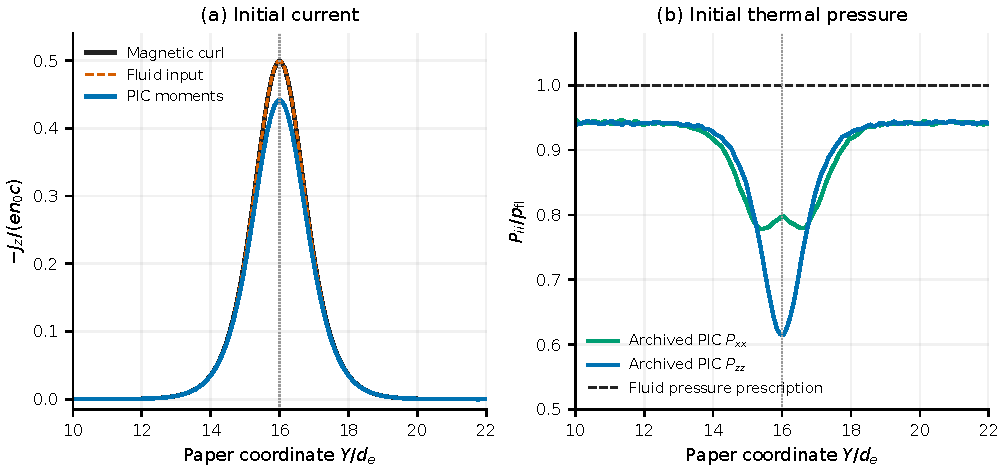
\includegraphics[width=\linewidth]{../figures/initial-state.pdf}
\caption{Reanalysis of the archived initial state near the lower sheet.
Left: the ordinary-velocity moment current differs from both the staggered
magnetic curl and the posted fluid prescription. Right: the local centered
pressure components, averaged in $x$ after centering, differ from the isotropic
fluid pressure. The profiles use the authors' archived diagnostics and
their published definitions~\cite{dataset}. The drawn fluid curves use the
initializer; the reloaded initial fluid output independently corroborates
them to roundoff. No new simulation is shown.}
\label{fig:initial-state}
\end{figure}

\begin{figure}[tbp]
\centering
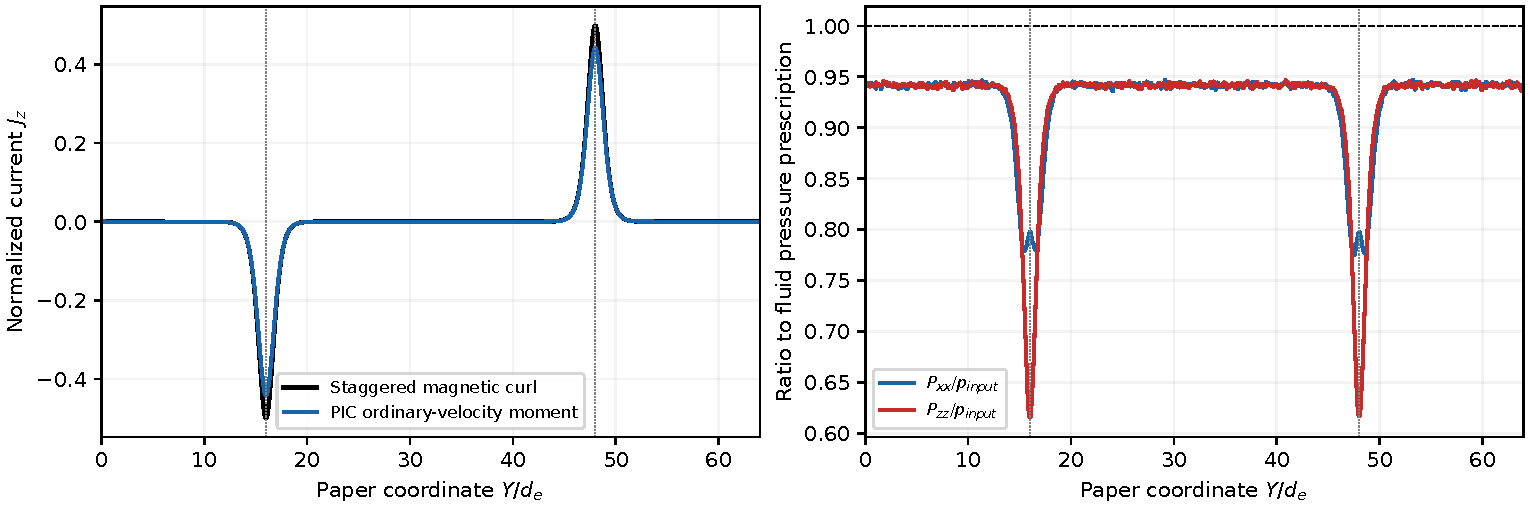
\includegraphics[width=\linewidth]{../figures/profile-sensitivity.pdf}
\caption{Full-domain, $x$-averaged archived PIC profiles at $t=0$, with both
current sheets visible. Left: physical moment current and the correctly
staggered magnetic curl. Right: velocity-covariance pressures divided by
the fluid pressure confirmed in the archived output. The figure extends the local view; it is neither
an independent simulation nor a native deposited-current diagnostic.}
\label{fig:full-profile}
\end{figure}
